In this chapter, the swarm algorithm is shown step by step
to solve the problem stated in chapter \ref{chap_problem}.
The module-level architecture of the onboard software based on this algorithm
is also designed and detailed.

\section{Swarm Algorithm Design}
\label{sec:alg_design}

\subsection{Dynamic Organisation of Tree Structure}

Before a group of UAVs is able to handle any task,
the UAVs should firstly organise themselves into a tree structure.
Since each UAV can be viewed as a single-node tree,
the problem can be viewed as building a single large tree from all existing small trees.
Before continuing, some terms, assumptions and key designs must be clarified.
\begin{remark}
    A swarm is defined as all the UAVs on the same tree.
    A sub-swarm is defined as all the UAVs on a sub-tree.
\end{remark}
In the context of this thesis, the term ``tree" is equivalent to the term ``swarm",
and they will be used interchangeably.
Similarly, term ``node" is sometimes used to refer to a UAV inside a swarm.
Building a single tree from small trees means building a single swarm from existing small swarms.
\begin{remark}
    Inside a tree, each child-parent node pair forms a connection.
    The child shall ensure that its distance from the parent is within communication range.
\end{remark}
A node may be in connection with multiple child nodes, but with at most one parent node.
For each child-parent pair, the child needs to track the parent
since it is responsible for keeping the communication range.
\begin{remark}
    Child node and parent node send connection messages to each other periodically,
    in order to exchange necessary data.
\end{remark}
To distinguish from the root UAV of the whole tree,
the root node of a sub-tree will be called the top node of that sub-tree.
\begin{remark}
    Inside a tree, for each child-parent node pair,
    the sub-tree topped by the child node is called a ``child sub-tree" of the parent node.
\end{remark}
\begin{remark}
    The size of a tree is the number of its nodes, i.e., the population of the swarm.
\end{remark}
\begin{remark}
    A set of existing trees can be strictly ordered by tree size and root node UAV ID.
\end{remark}
Trees of different sizes can be ordered by size.
Since UAV IDs are unique and comparable,
two trees of the same size can be distinguished and ordered by root node UAV ID.
\begin{remark}
    For a node on a tree, the ID sequence of all its ancestor nodes and itself
    is called the NID (meaning ``node ID") of the node.
\end{remark}
If the root node of a tree is UAV $U_i$, $U_i$ has child $U_j$,
and $U_j$ has child $U_k$, then the NID of $U_k$ is $[id_i, id_j, id_k]$.
An NID always starts with the ID of the root node of the tree.
The root node always knows its NID.
If a parent node knows its NID and sends its NID to its children,
the children will also known their NIDs.
\begin{remark}
    If every parent node sends its NID to its child nodes,
    recursively all nodes will known their correct NIDs.
\end{remark}
For a leaf node, i.e., node that has no children,
its sub-tree size is one, since the only member of the sub-swarm is itself.
For a parent node, if all its children know their respective sub-tree sizes
and send the data to the parent node,
the parent node can then calculate its own sub-tree size,
which is the sum of child sub-tree sizes plus one.
\begin{remark}
    If every child node sends its sub-tree size to its parent node,
    recursively all nodes will known their correct sub-tree sizes.
\end{remark}
For the root node, its sub-tree size is also the size of the whole tree.
\begin{remark}
    If every parent node sends tree-size data to its child nodes,
    recursively all nodes will known the correct tree size.
\end{remark}
The ultimate purpose of a swarm is to carry out tasks assigned by GCS.
For any swarm member, it may be handling some task, or it may be in free state.
\begin{remark}
    The ``current task ID" of a UAV is denoted by the $tid$ of the task,
    or is $None$ if the UAV is free.
\end{remark}
In order for the UAVs to discover each other and to obtain the status of each other,
they need to broadcast their information to nearby UAVs.
\begin{remark}
    A UAV broadcasts its NID, position, velocity, swarm size and current task ID periodically.
\end{remark}

Now the basic characteristics of a swarm are established,
and a UAV knows well about other UAVs in its neighbourhood. 
Initially, each UAV is a single-node tree.
To build a single tree from multiple existing trees,
two ideas are feasible: swarm-merging and swarm-switching.
\begin{itemize}
  \item Swarm-merging.
  For a swarm, if there are bigger other swarms nearby,
  the root node, leading the whole current swarm, joins the biggest swarm.
  \item Swarm-switching.
  For a UAV in a swarm, if there are bigger other swarms nearby,
  the UAV, leading its sub-swarm, leaves the current swarm and joins the biggest swarm.
\end{itemize}

In swarm-merging method, a smaller tree joins a bigger tree as a whole.
Trees are stable.
Existing trees will not collapse during merging process unless failure occurs.
In swarm-switching method, trees are not stable since nodes may leave at any time.
However, it's hard for swarm-merging method to handle the case
where the nearby biggest swarm is found by a non-root node,
but is out of the communication range of the root node.
Whereas for tree-switching method,
the node which finds the biggest swarm just joins the new swarm,
and other nodes of the old swarm will almost certainly find the new swarm
since they are at least in the communication range of that switching node.

The swarm-switching method is adopted.
The pseudocode is shown in algorithm \ref{alg:swarm-switching}.
The variable $self$ in the algorithm refers to the UAV that runs the algorithm.
The algorithm is only run when a UAV is free, i.e., when its current task ID is $None$.
The root node ID is used to tell which tree a node is currently on,
it is contained in the NID of a node.
When comparing two swarms, the swarm of bigger size is ordered before the one of smaller size.
If two swarms are of the same size,
the swarm with smaller root ID is ordered before the one with bigger root ID.

\begin{algorithm}
\caption{Swarm-switching algorithm.}
\label{alg:swarm-switching}
\begin{algorithmic}[1]
\Require $self$ is free
\Function{SwitchTree}{$self$}
\State $root\_self \gets self$.get\_root\_id()
\State $candidates \gets$ all nearby UAVs
\State $candidates$.filter\_by($candidate$ is free)
\State $candidates$.filter\_by($candidate$.get\_root\_id() $\neq root\_self$)
\State $candidates$.filter\_by(swarm of $candidate$ ordered before swarm of $self$)
\If{$candidates$ is not empty}
    \State $candidates$.sort\_by(ordering of their respective swarms)
    \State $new\_swarm\_root \gets candidates[0]$.get\_root\_id()
    \State $candidates$.filter\_by($candidate$.get\_root\_id() $= new\_swarm\_root$)
    \State $candidates$.sort\_ascending\_by(distance($candidate$, $self$))
    \State $self$.set\_parent($candidates[0]$)
\EndIf
\EndFunction
\end{algorithmic}
\end{algorithm}

In algorithm \ref{alg:swarm-switching},
after a UAV $U_i$ sets another UAV $U_j$ as its parent node,
$U_i$ should send a request message to $U_j$.
$U_j$ can accept the request,
or if $U_j$ is in inappropriate state,
it can reject the request by sending $U_i$ a reject message.
If $U_i$ receives a reject message,
it separates from $U_j$ and the sub-tree led by it becomes a new independent tree.

If all free UAVs within communication range keep running algorithm \ref{alg:swarm-switching},
they will eventually form a single tree.
Due to the latency of data flow inside a tree,
information stored by a node, such as swarm size, may not be updated timely.
Theoretically, this may cause nodes to join a tree which is not the biggest one.
However, information will eventually propagate throughout a tree,
and the algorithm is expected to converge.

\subsection{Task Coordination}

Tasks are handled hierarchically.
The root node divides the shape of a task into parts,
one for itself, and the others sent to its children.
Its children then repeat this process, until every node gets a portion of the shape.
Execution of a task means adjusting the velocity appropriately,
so the UAV flies onto its part of the shape, and stays there for a required time duration.

In this thesis, based on the context, the word ``task" may refer to three cases:
the task sent by the GCS to a swarm;
a portion of the task that is allocated to a sub-swarm;
a portion of the task that is allocated to a node.
The word ``sub-task" is also used to refer to the latter two cases.

When the UAVs are in free state, the swarm is not stable.
Nodes may join or leave a swarm.
It is hard for an unstable swarm to handle tasks properly.
So after a swarm receives a task,
it needs to firstly fix itself before it starts to handle the task.
An inner state is needed for every UAV to represent whether it has a task.
\begin{remark}
    The current task ID of a UAV is none $\iff$ the UAV is in state $Free$;
    the current task ID of a UAV is some $tid$ $\iff$ the UAV is in state $InTask$.
\end{remark}
\begin{remark}
    If a UAV is in state $InTask$, it shall not leave the swarm;
    it shall also reject any request that sets it as parent.
\end{remark}
It can be seen that if all members of a swarm is in $InTask$ state, the swarm is stable.
So after a task is received,
an approach is needed to transform the whole swarm into $InTask$ state.
\begin{remark}
    Based on the execution state of the task,
    $InTask$ state has three sub-states:
    $InTask(InProgess)$, $InTask(Success)$ and $InTask(Failure)$.
\end{remark}
\begin{remark}
    If a non-root UAV receives a task message sent by GCS,
    it relays the GCS task to its parent node.
    If root UAV receives a GCS task,
    it turns from $Free$ state into $InTask(InProgress)$ state.
\end{remark}
A child node can receive the current task ID of its parent node.
It changes its state according to this information.
\begin{remark}
    A child node turns into $Free$ state if the current task ID of its parent is $None$;
    and turns into $InTask(InProgress)$ state if the current task ID of its parent is some $tid$.
\end{remark}
All UAVs in a swarm will recursively align their $Free$/$InTask$ states with the root UAV.
After the root node receives a GCS task,
the whole swarm will gradually transform into $InTask(InProgress)$ state.
Before this alignment is complete,
the tree structure may change,
besides, the swarm size and sub-swarm size data stored by a UAV may be incorrect,
so task division is not possible.
Note that, for non-root nodes,
$InTask$ means it has received the task ID,
but may or may not have actually received a sub-task.

After the root node turns into $InTask(InProgress)$,
it needs to know whether all the other UAVs have finished aligning their states,
in order to start to divide the task and allocate sub-tasks.
In addition, once a task is fully divided and allocated to every node,
the root node needs to know the sub-task results of all other UAVs,
in order to decide the final result of the task.
\begin{remark}
    A node in $InTask(InProgress)$ turns into $InTask(Success)$
    if all nodes in its sub-tree succeeded in executing the task;
    A node in $InTask(InProgress)$ turns into $InTask(Failure)$
    if any node in its sub-tree failed in executing the task.
\end{remark}

Again, those information can be collected in a recursive way.
For this purpose, besides the state of a node itself,
the overall state of the sub-tree topped by the node is also needed.
\begin{remark}
    At any time point, a sub-swarm is in one of the six task states:
    $None$, $Recv$, $Algn$, $Allc$, $Succ$, and $Fail$.
\end{remark}
The meaning of the six task states are explained in table \ref{tbl:subswm_tsk_state}.
The top node of a sub-tree is responsible for
calculating the sub-swarm task state and sending it to its parent node.
The calculation process is shown in algorithm \ref{alg:subswarm-tsk-state}.
It is seen that the top node needs data from its children to do the calculation,
which means recursion.
A leaf node has no children.
Once it receives a task ID and turns into $InTask(InProgress)$,
its sub-tree, which contains only itself, is in task state $Algn$.
The node then reports $Algn$ to its parent.
If all children of the parent report $Algn$,
the parent knows that all its child sub-trees have been aligned to $InTask$,
and the parent's sub-tree is in task state $Algn$.
Recursively, the root node will eventually know that the whole swarm has been aligned.
Sub-task results are propagated up the tree in a similar way.

\begin{table}[htbp]
\centering
\caption[Sub-swarm task states.]
{The meaning of the six task states of a sub-swarm.}
\label{tbl:subswm_tsk_state}
\begin{tabular}{c|p{0.75\linewidth}}
  \hline
  $None$ & The top node is in $Free$ state. \\
  \hline
  $Recv$ & The top node has received the task ID and is in $InTask(InProgress)$,
           but has not confirmed that all the other nodes of the sub-tree are in $InTask$. \\
  \hline
  $Algn$ & The top node has confirmed that all nodes of the sub-tree are in $InTask$,
           and it has not received a sub-task from its parent. \\
  \hline
  $Allc$ & The top node has confirmed that all nodes of the sub-tree are in $InTask$,
           and it has received a sub-task from its parent. \\
  \hline
  $Succ$ & The top node finds that all nodes of the sub-tree have succeeded. \\
  \hline
  $Fail$ & The top node finds that at least one node of the sub-tree has failed. \\
  \hline
\end{tabular}
\end{table}

\begin{algorithm}
\caption{The process of the top node calculating the sub-swarm task state.}
\label{alg:subswarm-tsk-state}
\begin{algorithmic}[1]
\Function{CalculateSubswarmTaskState}{$self$}
\State $state\_self \gets self$.get\_node\_state()
\If{$state\_self$ = $Free$}
    \State \Return $None$
\ElsIf{$state\_self$ = $InTask(Success)$}
    \State \Return $Succ$
\ElsIf{$state\_self$ = $InTask(Failure)$}
    \State \Return $Fail$
\Else \Comment{$state\_self$ = $InTask(InProgress)$}
    \If{any child sub-swarm in $None$ or $Recv$}
        \State \Return $Recv$
    \Else \Comment{No children, or all child sub-swarms have been aligned}
        \If{$self$ has received a sub-task}
            \State \Return $Allc$
        \Else
            \State \Return $Algn$
        \EndIf
    \EndIf
\EndIf
\EndFunction
\end{algorithmic}
\end{algorithm}

With the sub-swarm task states defined above and algorithm \ref{alg:subswarm-tsk-state},
it is easy to figure out the complete state transition conditions of a node
and what a node should do in each of the states.
\begin{remark}
If all children of the root node report sub-tree task state $Algn$,
then all nodes are in $InTask$, and the task can be divided and allocated layer by layer.
\end{remark}
When a node with $N_c$ children divides a received task,
the task is divided into $N_c + 1$ sub-tasks, one for itself and $N_c$ for its child sub-trees.
The weight of each sub-task shall be proportional to the number of UAVs executing it.
\begin{remark}
If all children of a node report sub-tree task state $Allc$,
it means the sub-task allocation process of that node is finished.
\end{remark}
\begin{remark}
If a node fails a task,
or if it loses connection with a child which is in $InTask$ state,
or if any of its children reports sub-tree task state $Fail$,
the node turns into $InTask(Failure)$ state.
\end{remark}
\begin{remark}
If a node succeeds in a task, i.e., has stayed long enough on some shape,
and all its children report sub-tree task state $Succ$,
the node turns into $InTask(Success)$ state.
\end{remark}
If the root node turns into $InTask(Failure)$ or $InTask(Success)$ state,
the whole GCS task is failed or successful,
and the root node will turn into $Free$ to wait for the next GCS task.

\begin{figure}[htbp]
  \centering
  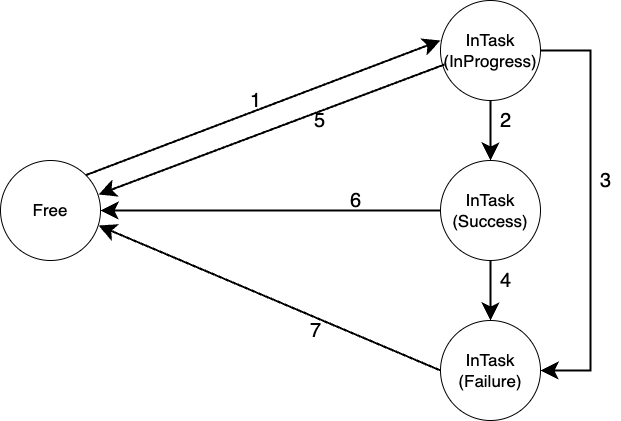
\includegraphics[width=0.7\linewidth]{rsc/node_state_machine.png}
  \caption[State transitions of a node.]
  {State transition conditions for a node.
  [1] The root node receives a GCS task;
  or a non-root node receives the current task ID $tid$ from its parent.
  [2] A node has succeeded and all its children report sub-swarm task state $Succ$.
  [3, 4] A node has failed,
  or it loses connection with a child which is in $InTask$ state,
  or any of its children reports sub-swarm task state $Fail$.
  [5] A non-root node receives the current task ID $None$ from its parent.
  [6] A non-root node receives the current task ID $None$ from its parent;
  or the root node decides that the whole task has succeeded.
  [7] A non-root node receives the current task ID $None$ from its parent;
  or the root node decides that the whole task has failed.
  }
  \label{fig:node_state_machine}
\end{figure}

\begin{table}[htbp]
\centering
\caption[States of a node.]
{What a node does in different states.}
\label{tbl:node_state_doing}
\begin{tabular}{c|p{0.6\linewidth}}
  \hline
  $Free$ & A node tries to join a bigger swarm. \\
  \hline
  $InProgress(InProgress)$ & A node waits until all its children are in $InTask$ state
            (i.e., all children report sub-tree task state $Algn$)
            and a task has been allocated to it;
            then it divides the task,
            allocates sub-tasks, and executes its own sub-task. \\
  \hline
  $InProgress(Success)$ & The root node switches to $Free$ state;
                          a non-root node waits for its parent to change state. \\
  \hline
  $InProgress(Failure)$ & The root node switches to $Free$ state;
                          a non-root node waits for its parent to change state. \\
  \hline
\end{tabular}
\end{table}

\begin{figure}[htbp]
  \centering
  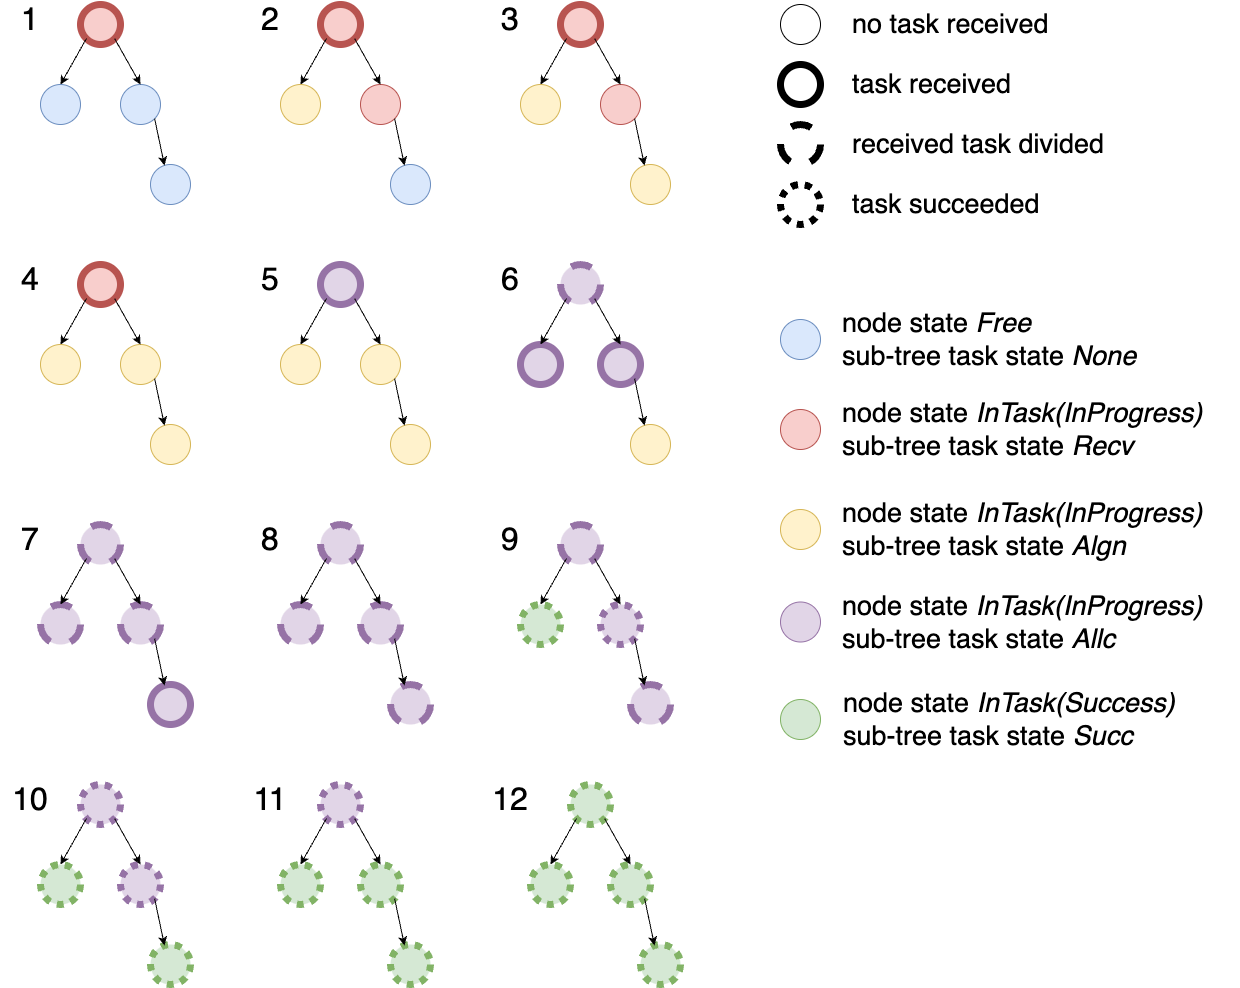
\includegraphics[width=0.9\linewidth]{rsc/task_state_transition.png}
  \caption[An example of state transitions of a swarm.]
  {An example of state transitions of a 4-UAV swarm during a task. \\
  Image 1 shows the root have received a GCS task. \\
  Image 1-3 depict how the nodes align their states with the root. \\
  Image 3-5 depict how the information of alignment completion propagates up the tree. \\
  Image 6-8 depict how each node divides and allocates tasks down the tree. \\
  Image 9 and 10 show nodes finish their tasks. \\
  Image 10-12 depict how the root knows that all nodes have succeeded.
  }
  \label{fig:swarm_state_transition}
\end{figure}

Figure \ref{fig:node_state_machine} shows the state transition conditions of a node.
Table \ref{tbl:node_state_doing} summarises what a node shall do in each of the states.
Figure \ref{fig:swarm_state_transition} gives an example of
how node state changes in a swarm during a task.

It is worth noticing that, for a task with shape $S$ and time duration $\Delta t$,
the root node in $InTask(Success)$ state only means that
all nodes have stayed on $S$ for at least $\Delta t$,
however, the overlapping part of their stay duration may not be long enough.
This problem is ignored,
for it deviates from the main focus of this thesis and requires complex algorithm to solve.

\section{Velocity Control}

Velocity control is related to formation control and path planning.
To maintain the connection with the parent node,
a UAV also needs to track its parent.
To execute a task,
a UAV needs appropriate velocity to move around or to stay at some position.
Besides, collision with other UAVs shall be avoided.
All these requirements contribute to the complexity of the calculation of velocity.
A behavioural approach is adopted.
The structural design of velocity control is illustrated in figure \ref{fig:v_ctrl}.

\begin{figure}[htbp]
  \centering
  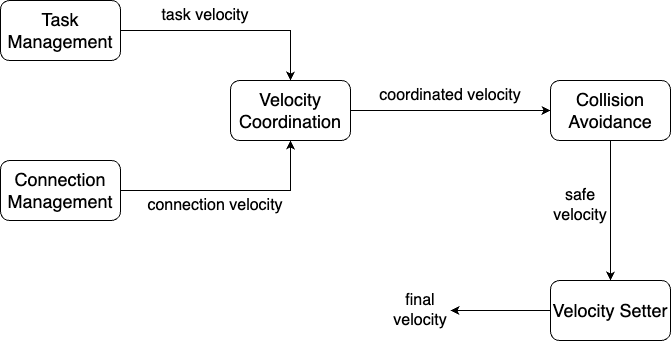
\includegraphics[width=0.8\linewidth]{rsc/velocity_control_structure.png}
  \caption
  {The structure of velocity control.}
  \label{fig:v_ctrl}
\end{figure}

If a UAV has a task, the task velocity is needed by task execution.
For non-root nodes,
the connection velocity constrains the UAV from flying too far away from its parent,
so as to maintain the connection with its parent.
These two velocities goes into a coordinator, which generates a coordinated velocity.
The basic idea of the velocity coordination is,
task velocity dominates if the parent is within a safe distance,
and connection velocity dominates if the parent is on the verge of losing connection.
The collision avoidance module takes the coordinated velocity as input
applies modifications to prevent collisions with nearby UAVs,
and outputs a safe velocity.
The velocity setter corresponds to the flight control module on a real UAV.
It takes the safe velocity,
clamps it if it exceeds the maximum UVA speed $v_{max}$,
and sets it as the final desired velocity.

Figure \ref{fig:v_ctrl} shows only the idea and structure of velocity control.
The exact algorithms of each part are up to the implementation.

\section{Software Architecture Design}
\label{sec:sft_arch}

To run and test the designed swarm algorithm on a UAV,
a piece of onboard software which implements the algorithm is needed.
In this section, a top-down modular architecture of the software is designed.

\begin{figure}[htbp]
  \centering
  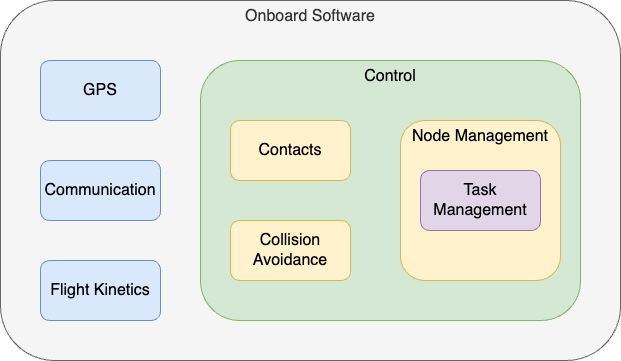
\includegraphics[width=0.8\linewidth]{rsc/software_architecture.png}
  \caption
  {The architecture of the onboard software.}
  \label{fig:software_arch}
\end{figure}

As shown in figure \ref{fig:software_arch},
the top-level modules are GPS module, Communication module,
Flight Kinetics module, and Control module.
Among them, the Control module implements the swarm algorithm,
while all the other three are hardware interfaces
that interact with sensors, radio frequency (RF) devices, or actuators.
Since this thesis runs simulations, there is no hardware,
so the three modules actually interact with simulation infrastructure.

The Control module is where the designed swarm algorithm is implemented.
It contains three child modules:
Contacts module, Collision Avoidance module, and Node Management module.
The Contacts module monitors nearby UAVs that are in communication range.
The Collision Avoidance module prevents collision with other UAVs by adjusting velocity.
The Node Management module handles connections with parent and children,
and manages node state transitions.
It further contains the Task Management module, which divides and executes tasks.

\begin{table}[htbp]
\centering
\caption[Modules of onboard software.]
{The functionality of each module.}
\label{tbl:modules}
\begin{tabular}{c|p{0.7\linewidth}}
  \hline
  GPS & Interface to the GPS sensor. Provides position information to other modules.  \\
  \hline
  Communication & Interface to the RF device.
                  Provides received messages from nearby UAVs to other modules,
                  and sends messages generated by other modules to nearby UAVs. \\
  \hline
  Flight Kinetics & Interface to the flight control system.
                    Sets the UAV velocity to the value required by other modules.
                    Corresponds to the ``Velocity Setter" in figure \ref{fig:v_ctrl}. \\
  \hline
  Control & Implements the swarm algorithm. \\
  \hline
  Contacts & Monitors all the other UAVs within communication range.
             Provides notice when a UAV loses contact. \\
  \hline
  Node Management & Manages the connections with parent and children,
                    and manages the transitions of node states
                    (figure \ref{fig:node_state_machine}).
                    This is the core module of the swarm algorithm.
                    Responsible for generating connection velocity and
                    coordinated velocity (figure \ref{fig:v_ctrl}). \\
  \hline
  Task Management & Manages a received task.
                    Responsible for dividing a task
                    and generating task velocity (figure \ref{fig:v_ctrl}). \\
  \hline
  Collision Avoidance & Prevents the UAV from colliding with neighbour UAVs
                        (figure \ref{fig:v_ctrl}). \\
  \hline
\end{tabular}
\end{table}

Table \ref{tbl:modules} lists the functionality of each module.
Figure \ref{fig:seq_sftwr} shows the sequence diagram of the onboard software.
It is a single-thread design.
The main part of the software is an infinite loop.
Inside the body of the main loop, the Control module is responsible for
updating the inner status of the UAV and controlling the UAV.
The detailed sequence diagram of the Control module
is shown in figure \ref{fig:seq_control}.
The detailed sequence diagram of the Node Management module
is shown in figure \ref{fig:seq_nm}.
These sequence diagrams show how the modules carry out the designed algorithm.

\begin{figure}[htbp]
  \centering
  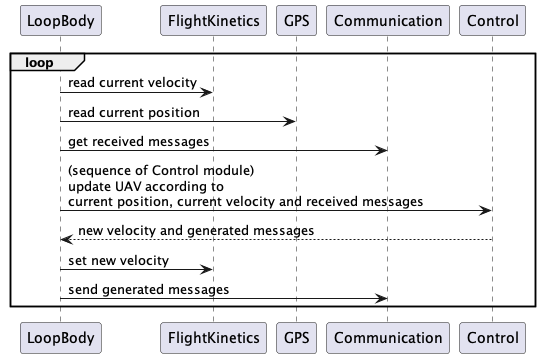
\includegraphics[width=0.8\linewidth]{rsc/astro_sequence.png}
  \caption
  {Sequence diagram of the onboard software.}
  \label{fig:seq_sftwr}
\end{figure}

\begin{figure}[htbp]
  \centering
  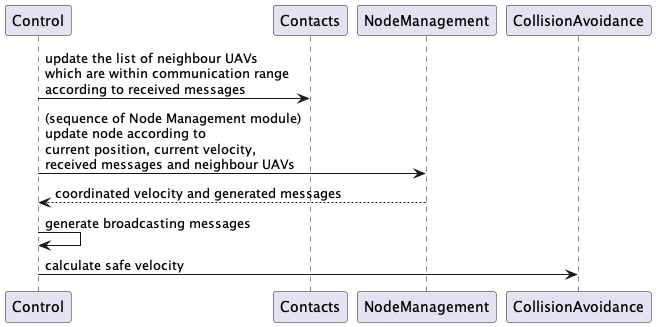
\includegraphics[width=0.9\linewidth]{rsc/control_sequence.png}
  \caption
  {Sequence diagram of the Control module.}
  \label{fig:seq_control}
\end{figure}

\begin{figure}[htbp]
  \centering
  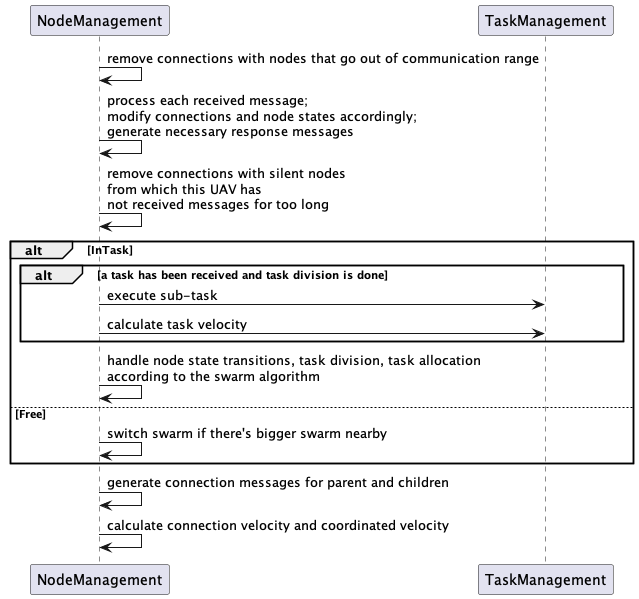
\includegraphics[width=0.9\linewidth]{rsc/nm_sequence.png}
  \caption
  {Sequence diagram of the Node Management module.}
  \label{fig:seq_nm}
\end{figure}